\subsubsection{Обход и правила}

На входе имеем $roren$ граф $G$. Обозначения:\\
$PD$ - ParDo, $F$ - Flatten, $Gbk$ - GroupByKey\\
$\$Transform^{\pm}$ -  Transform с сохранением сортировки или без\\
$\pm$ - вход, сортированный или нет\\
$\$Transform^{*}$ - оригиальный Transform из $roren$, имеющий один вход\\
Алгоритм будет опираться на правила (рис.~\ref{fig:rule1}), которые позволяют объединять Transform-ы в одну операцию для дальнешего запуска YT операций.\\
\begin{figure}[h]
    \centering
    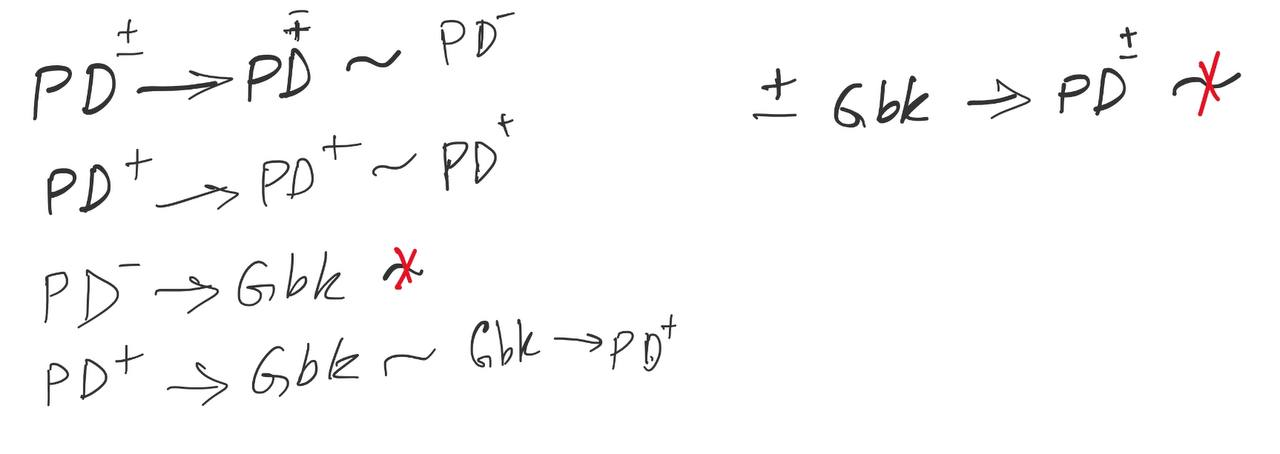
\includegraphics[width=0.7\textwidth]{img/rule1.jpeg}
    \caption{Правила roren $\xrightarrow{}$ roren}
    \label{fig:rule1}
\end{figure}

\begin{algo}
Сначала перестроим граф $G$ по правилу $F \xrightarrow{} \$Transform* \sim \$Transform$, где $Transform$ - это некоторое преобразование, которое после перестройки может иметь несколько входов (рис.~\ref{fig:flatten}).\\
\begin{figure}[h]
    \centering
    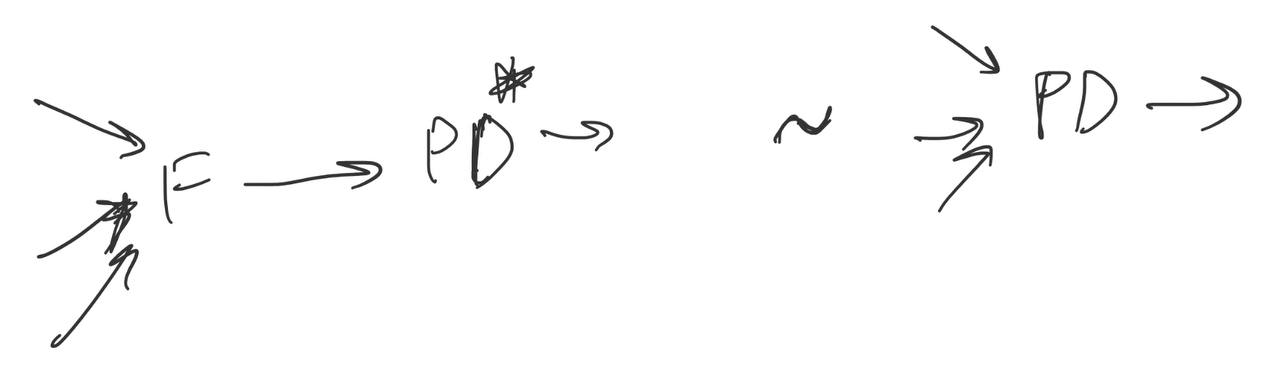
\includegraphics[width=0.5\textwidth]{img/flatten.jpeg}
    \caption{Преобразование с Flatten}
    \label{fig:flatten}
\end{figure}

Построим слоистую сеть $R$ по $G$ (рис.~\ref{fig:net}).\\
\begin{figure}[h]
    \centering
    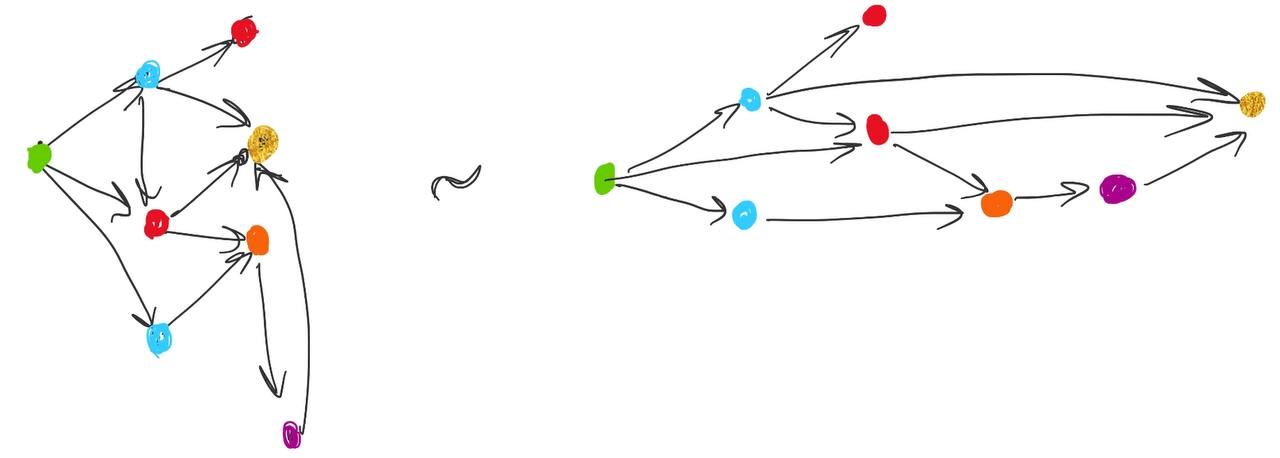
\includegraphics[width=0.8\textwidth]{img/net.jpeg}
    \caption{Построение слоистой сети}
    \label{fig:net}
\end{figure}

Теперь будем проходить по $R$. Шаг обхода будет состоять из двух стадий: collapse и expand. На стадии collapse некоторые вершины сливаются, на стадии expand новые вершины добавляются в рассмотрение. Обход будем делать по слоям, рассматривая текущий и следующий, по ходу присваивая вершинам цвета:\\
\begin{itemize}
    \item черные - ещё не посещенные вершины, на слоях отличных от текущего и следующего,
    \item оранжевые - посещенные вершины, на текущем слое или на предыдущих слоях, если есть ребро в черную вершину,
    \item красные - не посещенные вершины, находящиеся на следующем слое,
    \item зеленые - посещенные вершины, которые больше не будут участовать в слиянии.
\end{itemize}
При старте обхода помечаем первый слой оранжевым цветом, второй слой красным.\\
На произвольном шаге алгоритма рассматриваем каждую из оранжевых вершин отдельно. Сначала идет стадия collapse. На данном этапе может возникнуть 2 типа коллизий (рис.~\ref{fig:collision}), которые можно пытаться разрешать, но мы не будем...\\
\begin{figure}[h]
    \centering
    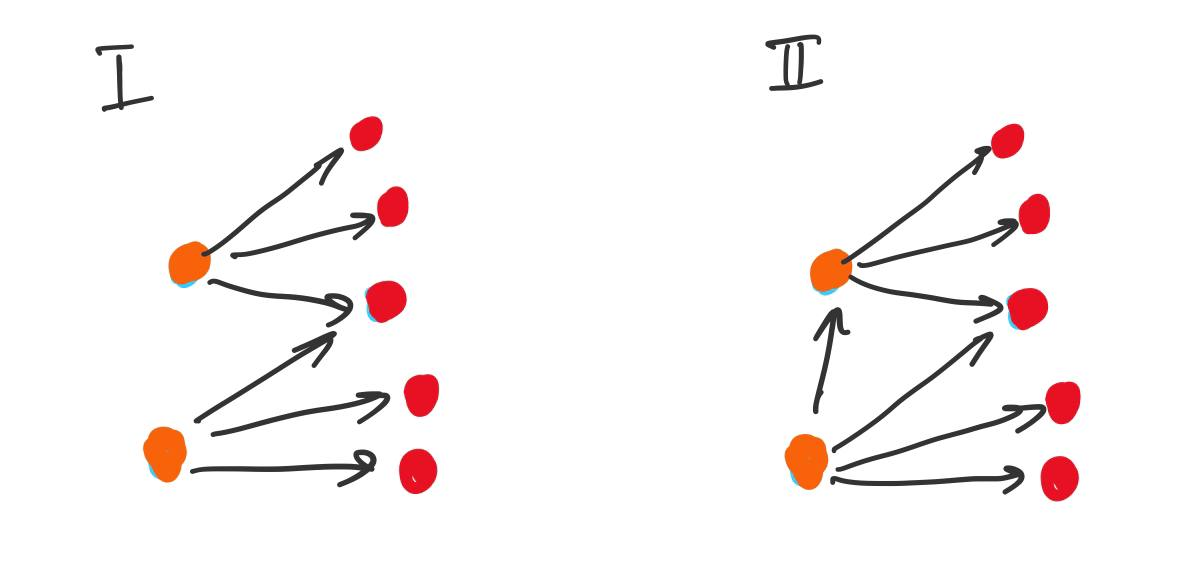
\includegraphics[width=0.7\textwidth]{img/collision.jpeg}
    \caption{Типы коллизий}
    \label{fig:collision}
\end{figure}

Для вершин, в которых не возникает коллизий, применяя правила roren $\xrightarrow{}$ roren, можно влить красную вершину в оранжевую.\\
После начинается стадия expand, оставшиеся красные вершины окрашиваются в оранжевый, текущий слой продвигается вперед. Сейчас оранжевые вершины с прошлого слоя могут стать зелеными, в случае если все ребра входят в оранжевые вершины.\\
Пример обхода приведен на рис.~\ref{fig:algo}.\\
\begin{figure}[h]
    \centering
    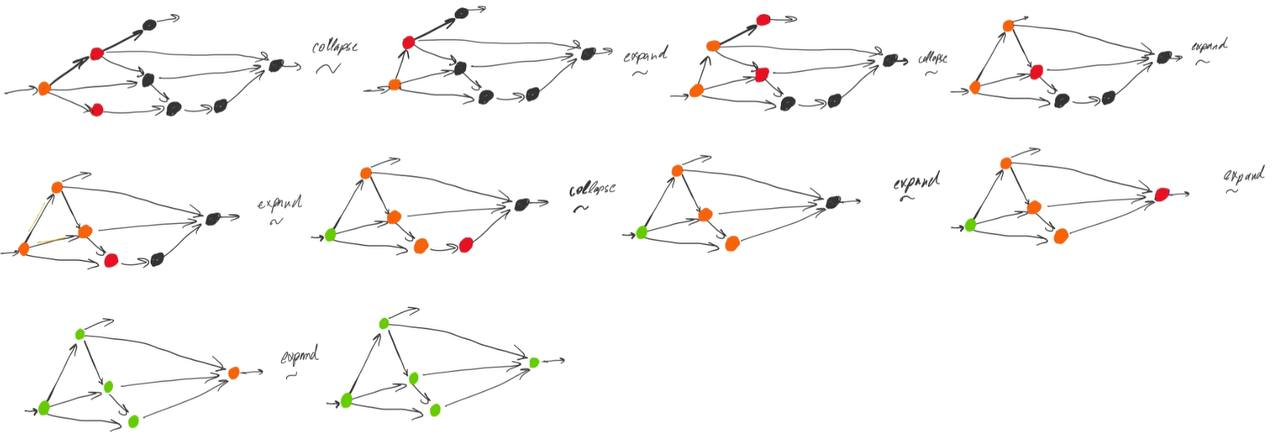
\includegraphics[width=\textwidth]{img/algo.jpeg}
    \caption{Пример обхода}
    \label{fig:algo}
\end{figure}

После того, как завершился обход по сети $R$. Можно перевести граф в операции Map, Reduce и MapReduce по правилам roren $\xrightarrow{}$ YT (рис.~\ref{fig:rule2}).\\
\end{algo}

\begin{figure}[h]
    \centering
    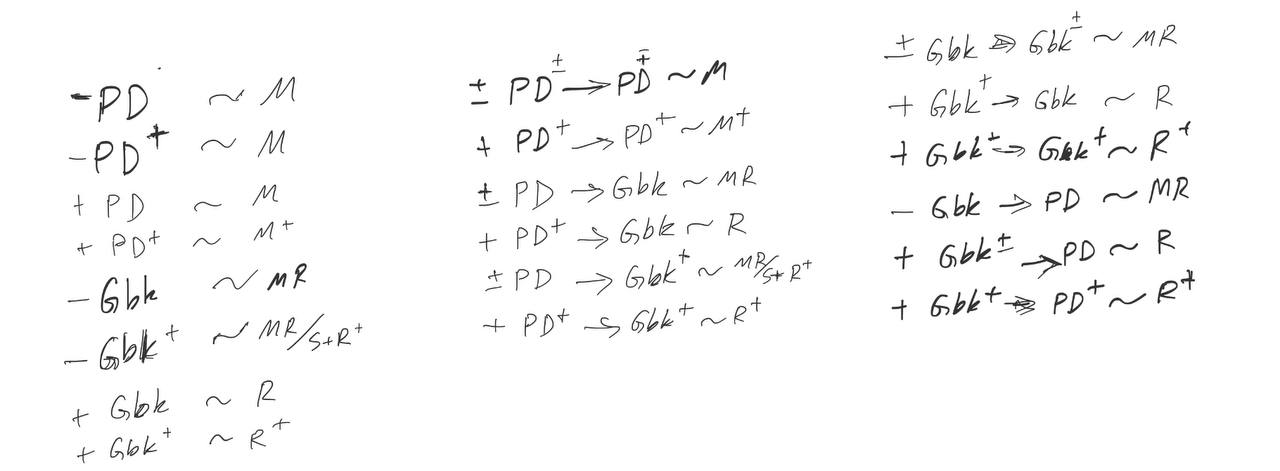
\includegraphics[width=\textwidth]{img/rule2.jpeg}
    \caption{Правила roren $\xrightarrow{}$ YT}
    \label{fig:rule2}
\end{figure}

\begin{comment}
На самом деле, в алгоритме есть несколько точек кастомизации поведения.\\
\begin{itemize}
\item Мы можем пытаться разрешать коллизии (рис.~\ref{fig:collision}): для первого типа сливать две оранжевые вершины, для второго придумать правила для "треугольников".
\item После преобразований размер данных по ключу может сильно меняться: уменьшаться, если трансформ фильтрует данные, увеличиваться, если дробит.
\item Можно сливать независимые ветки графа, но стоит думать об отсутствии параллельности исполнения в данном случае.
\item У операций в качестве атрибутов могут быть выставлены лимиты на ресурсы, которые есть возможность учитывать при слияниях.
\item Прежде чем применять во всех местах правила слияния с учетом сортированности, можно сделать предпроход и понять до каких входом прокидывается сортированность.
\item Кажется, что coGbk пока нельзя средствами YT выразить; Combine распадается в два Reduce; Flatten, после которого не шло никаких Transform, станет YT Merge-ом.
\item Если у Transform-а есть side выход и ребро в другой Transform, то можно не делать временную таблицу.
\end{itemize}
\end{comment}
